\section{Merger of the two projects}

\begin{frame}{Merger of the two projects -- roadmap}
	\begin{block}{What we got}
		\begin{itemize}
			\item Pairwise shortest paths between stations.
			\item Series of travels from one point to another.
		\end{itemize}
	\end{block}
	\begin{alertblock}{What we want}
		\begin{itemize}
			\item Retrieve the itinerary for each travel !
		\end{itemize}
	\end{alertblock}
\end{frame}

\begin{frame}{Merger of the two projects -- illustration}
	\begin{figure}
		\centering
		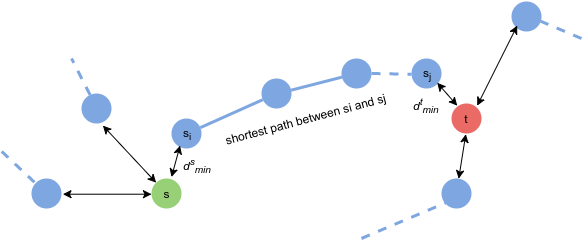
\includegraphics[width=\linewidth]{images/shortest_path.png}
		\caption{Computation of point-to-point shortest paths}
	\end{figure}
\end{frame}
\begin{frame}{Merger of the two projects -- result}
	\begin{figure}
		\centering
		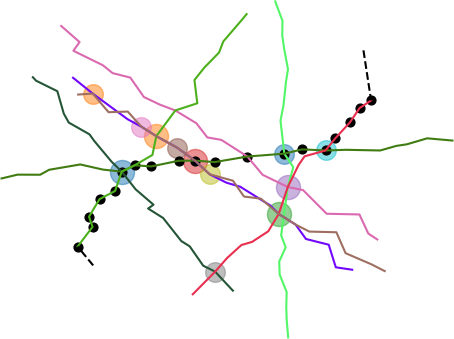
\includegraphics[width=0.7\linewidth]{images/net_8.png}
		\caption{Shortest path -- compute point to point shortest path using SymPy and NetworkX}
	\end{figure}
\end{frame}
\begin{frame}{Conclusion}
	\begin{itemize}
		\item Complex and quite ``realistic'' city with many adjustable parameters.
		\item But define ``realistic'' ? Which metric could we use ?
		\item Possible refinements : animated viz', wider range of public transport, wider range of socio-professional categories...
	\end{itemize}
	
\end{frame}